
\documentclass{beamer}
\usepackage[utf8]{inputenc}

\usetheme{Madrid}
\usecolortheme{default}
\usepackage{amsmath,amssymb,amsfonts,amsthm}
\usepackage{txfonts}
\usepackage{tkz-euclide}
\usepackage{listings}
\usepackage{adjustbox}
\usepackage{array}
\usepackage{tabularx}
\usepackage{gvv}
\usepackage{lmodern}
\usepackage{circuitikz}
\usepackage{tikz}
\usepackage{graphicx}

\setbeamertemplate{page number in head/foot}[totalframenumber]

\usepackage{tcolorbox}
\tcbuselibrary{minted,breakable,xparse,skins}



\definecolor{bg}{gray}{0.95}
\DeclareTCBListing{mintedbox}{O{}m!O{}}{%
  breakable=true,
  listing engine=minted,
  listing only,
  minted language=#2,
  minted style=default,
  minted options={%
    linenos,
    gobble=0,
    breaklines=true,
    breakafter=,,
    fontsize=\small,
    numbersep=8pt,
    #1},
  boxsep=0pt,
  left skip=0pt,
  right skip=0pt,
  left=25pt,
  right=0pt,
  top=3pt,
  bottom=3pt,
  arc=5pt,
  leftrule=0pt,
  rightrule=0pt,
  bottomrule=2pt,
  toprule=2pt,
  colback=bg,
  colframe=orange!70,
  enhanced,
  overlay={%
    \begin{tcbclipinterior}
    \fill[orange!20!white] (frame.south west) rectangle ([xshift=20pt]frame.north west);
    \end{tcbclipinterior}},
  #3,
}
\lstset{
    language=C,
    basicstyle=\ttfamily\small,
    keywordstyle=\color{blue},
    stringstyle=\color{orange},
    commentstyle=\color{green!60!black},
    numbers=left,
    numberstyle=\tiny\color{gray},
    breaklines=true,
    showstringspaces=false,
}
\begin{document}

\title 
{9.2.33}
\date{September 14,2025}


\author 
{EE25BTECH11065-Yoshita J}






\frame{\titlepage}
\begin{frame}{Question}
Find the area of the region enclosed by the parabola \(x^{2}=y\) and the line \(y=x+2\), using the matrix formulation of conics and the intersection-of-line-with-conic formula.\\

\end{frame}


\begin{frame}{Theoretical Solution}
The given ellipse can be expressed as conics with parameters,
\begin{align*}
\vec{x}^{\top}\vec{V}\vec{x}+2\vec{u}^{\top}\vec{x}+f=0,\qquad 
\vec{x}=\myvec{x\\y}.
\end{align*}
where,
\begin{align}
\vec{V}=\myvec{1 & 0\\0 & 0},\qquad
\vec{u}=\myvec{0\\-\tfrac{1}{2}},\qquad
f=0.
\end{align}

The line parameters are 
\begin{align*}
\vec{x}=\vec{h}+\kappa\,\vec{m},\ \kappa\in\mathbb R.
\end{align*}
where,
\begin{align}
\vec{h}=\myvec{0\\2},\qquad \vec{m}=\myvec{1\\1}.
\end{align}

\end{frame}

\begin{frame}{Theoretical Solution}
Substituting the given parameters to find the intersection point,
\begin{align}
\kappa=\frac{1}{\vec{m}^{\top}\vec{V}\vec{m}}\Big(
-\,\vec{m}^{\top}(\vec{Vh}+\vec{u})
\pm
\sqrt{\big(\vec{m}^{\top}(\vec{Vh}+\vec{u})\big)^{2}
-\,g(\vec{h})\;(\vec{m}^{\top}\vec{V}\vec{m})}
\Big),
\end{align}
where 
\begin{align}
g(\vec{h})=\vec{h}^{\top}\vec{V}\vec{h}+2\vec{u}^{\top}\vec{h}+f.
\end{align}
Solving,
\begin{align}
\vec{m}^{\top}\vec{V}\vec{m}
=\myvec{1 & 1}\myvec{1 & 0\\0 & 0}\myvec{1\\1}
=\myvec{1 & 1}\myvec{1\\0}=1.
\end{align}

\begin{align}
\vec{Vh}+\vec{u}
=\myvec{1 & 0\\0 & 0}\myvec{0\\2}
+\myvec{0\\-\tfrac{1}{2}}
=\myvec{0\\-\tfrac{1}{2}}.
\end{align}

\end{frame}

\begin{frame}{Theoretical Solution}
\begin{align}
\vec{m}^{\top}(\vec{Vh}+\vec{u})
=\myvec{1 & 1}\myvec{0\\-\tfrac{1}{2}}=-\tfrac{1}{2}.
\end{align}

\begin{align}
g(\vec{h})
=\vec{h}^{\top}\vec{V}\vec{h}+2\vec{u}^{\top}\vec{h}
=0+2\myvec{0 & -\tfrac{1}{2}}\myvec{0\\2}=-2.
\end{align}

Now the discriminant,
\begin{align}
\big(\vec{m}^{\top}(\vec{Vh}+\vec{u})\big)^{2}
-\,g(\vec{h})\,(\vec{m}^{\top}\vec{V}\vec{m})
=\left(-\tfrac{1}{2}\right)^{2}-(-2)\cdot 1
=\tfrac{1}{4}+2=\tfrac{9}{4},
\end{align}
so 
\begin{align}
\sqrt{\cdot}=\tfrac{3}{2}.
\end{align}

\end{frame}

\begin{frame}{Theoretical Solution}
Hence
\begin{align}
\kappa=\; -(-\tfrac{1}{2})\pm \tfrac{3}{2}
=\tfrac{1}{2}\pm \tfrac{3}{2}\quad\Longrightarrow\quad
\kappa_{1}=2,\ \kappa_{2}=-1.
\end{align}

Points of intersection,
\begin{align}
\vec{x}_{i}=\vec{h}+\kappa_{i}\vec{m}
\end{align}
\begin{align}
\vec{x}_{1}=\myvec{0\\2}+2\myvec{1\\1}=\myvec{2\\4},\qquad
\vec{x}_{2}=\myvec{0\\2}-1\myvec{1\\1}=\myvec{-1\\1}.
\end{align}

Thus the intersection points are 
\begin{align}
\myvec{-1\\1} \quad \text{and} \quad \myvec{2\\4}.
\end{align}

\end{frame}

\begin{frame}{Theoretical Solution}
Area of the enclosed region,
\begin{align}
A=\int_{-1}^{2}\big[(x+2)-x^{2}\big]\,dx
=\frac{9}{2}.
\end{align}

Therefore the area of the region enclosed by \(x^2=y\) and \(y=x+2\) is
\begin{align*}
\boxed{\tfrac{9}{2}}
\end{align*}
\end{frame}
\begin{frame}[fragile]
    \frametitle{C Code}

    \begin{lstlisting}
#include <stdio.h>

double calculate_area() {
    double upper_bound_integral = (2.0 * 2.0 / 2.0) + (2.0 * 2.0) - (2.0 * 2.0 * 2.0 / 3.0);
    double lower_bound_integral = (-1.0 * -1.0 / 2.0) + (2.0 * -1.0) - (-1.0 * -1.0 * -1.0 / 3.0);
    return upper_bound_integral - lower_bound_integral;
}
    \end{lstlisting}
\end{frame}


\begin{frame}[fragile]
    \frametitle{Python Code}
    \begin{lstlisting}
import numpy as np
import matplotlib.pyplot as plt

def parabola(x):
    return x**2

def line(x):
    return x + 2

x_range = np.linspace(-3, 4, 400)
y_parabola = parabola(x_range)
y_line = line(x_range)

fig, ax = plt.subplots(figsize=(8, 6))

    \end{lstlisting}
\end{frame}

\begin{frame}[fragile]
    \frametitle{Python Code}
    \begin{lstlisting}
ax.plot(x_range, y_parabola, 'b-', label='$y = x^2$')
ax.plot(x_range, y_line, 'r-', label='$y = x + 2$')

x_fill = np.linspace(-1, 2, 100)
ax.fill_between(x_fill, parabola(x_fill), line(x_fill), color='gray', alpha=0.3, label='Area = 9/2')
    
intersection_points_x = [-1, 2]
intersection_points_y = [1, 4]
ax.plot(intersection_points_x, intersection_points_y, 'ko')

ax.text(-1, 1, ' (-1, 1)', verticalalignment='bottom', horizontalalignment='right')
ax.text(2, 4, ' (2, 4)', verticalalignment='bottom', horizontalalignment='left')


   
    \end{lstlisting}
\end{frame}

\begin{frame}[fragile]
    \frametitle{Python Code}
    \begin{lstlisting}
ax.set_title('Area Bounded by Parabola and Line')
ax.set_xlabel('X-axis')
ax.set_ylabel('Y-axis')
ax.grid(True, linestyle='--')
ax.legend()

ax.axhline(0, color='black', linewidth=0.5)
ax.axvline(0, color='black', linewidth=0.5)

ax.set_aspect('equal', adjustable='box')

plt.show()

   
    \end{lstlisting}
\end{frame}  


\begin{frame}{Plot}
    \centering
    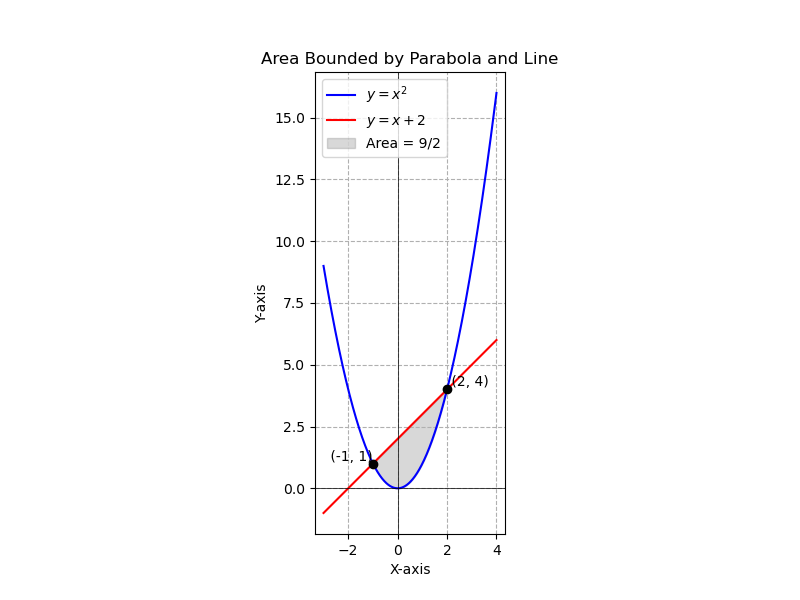
\includegraphics[width=\columnwidth, height=0.9\textheight, keepaspectratio]{figs/fig2.png}     
\end{frame}


\end{document}
